%Example of use of oxmathproblems latex class for problem sheets
\documentclass{oxmathproblems}

\usepackage{hyperref}
\usepackage{tikz}

%(un)comment this line to enable/disable output of any solutions in the file
\printanswers

%define the page header/title info
\oxfordterm{Term 1 2024}
\course{MRes in Soft Electronic Materials}
\sheetnumber{Solid State 1}
%\sheettitle{} %can leave out if no title per sheet

% add further contact details to footer if desired,
%e.g. email address, or name and email address
\contact{Set by Jarvist Moore Frost: jarvist.frost@imperial.ac.uk; please email with errata.}


\begin{document}
Reciprocal lattice

\begin{questions}

\miquestion
A two-dimensional rectangular crystal has a unit cell with sides $a_1
    = 0.468$~nm and $a_2 = 0.342$~nm. 

    \begin{parts}
\part
What is the area of the unit cell?
\part
Draw to scale a diagram of the reciprocal lattice of this crystal.
\part
Label the reciprocal lattice high-symmetry locations. 
\end{parts}

\begin{solution}
\begin{parts}
\part
The area of the unit cell is $a_1 \times a_2 = 0.468\text{ nm} \times 0.342\text{ nm} = 0.160\text{ nm}^2$

\part
The reciprocal lattice vectors are:
$b_1 = \frac{2\pi}{a_1} = 13.4\text{ nm}^{-1}$
$b_2 = \frac{2\pi}{a_2} = 18.4\text{ nm}^{-1}$

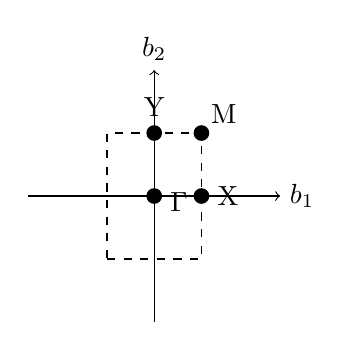
\begin{tikzpicture}[scale=0.4]
    % Draw axes
    \draw[->] (-4,0) -- (4,0) node[right] {$b_1$};
    \draw[->] (0,-4) -- (0,4) node[above] {$b_2$};
    
    % Draw unit cell boundaries (dashed)
    \draw[dashed] (-1.5,-2) -- (1.5,-2) -- (1.5,2) -- (-1.5,2) -- cycle;
    
    % Label high-symmetry points
    \node[circle,fill=black,inner sep=2pt] at (0,0) {};
    \node[right] at (0.2,-0.2) {$\Gamma$};
    
    \node[circle,fill=black,inner sep=2pt] at (1.5,0) {};
    \node[right] at (1.7,0) {X};
    
    \node[circle,fill=black,inner sep=2pt] at (0,2) {};
    \node[above] at (0,2.2) {Y};
    
    \node[circle,fill=black,inner sep=2pt] at (1.5,2) {};
    \node[above right] at (1.5,2) {M};
\end{tikzpicture}

\part
The high-symmetry locations are:
\begin{itemize}
    \item $\Gamma$ (origin): (0,0)
    \item X points: $(\pm\frac{b_1}{2},0)$
    \item Y points: $(0,\pm\frac{b_2}{2})$
    \item M points: $(\pm\frac{b_1}{2},\pm\frac{b_2}{2})$
\end{itemize}

The key thing to remember is that you always have the $\Gamma$ high symmetry location 
(the origin of reciprocal space), and that the other high symmetry locations depend on 
the space group - they are the edges of the Brillouin zone.
\end{parts}
\end{solution}
  

\miquestion
A collimated beam of monochromatic X-rays with wavelength $0.166$~nm is used to
exmaine the crystal.

\begin{parts}
\part
Calculate the Bragg condition from scattering from the $a_1$ plane of the
    crystal.
\part
Calculate the Bragg condition from scattering from the $a_2$ plane of the
    crystal.
\part
Draw a diagram showing the expected Bragg peaks from this crystal, plotting as
a function of $2\theta$. 
\end{parts}

\begin{solution}
We can use Bragg's law to answer this question.

This is a simple version of the standard diagram, 

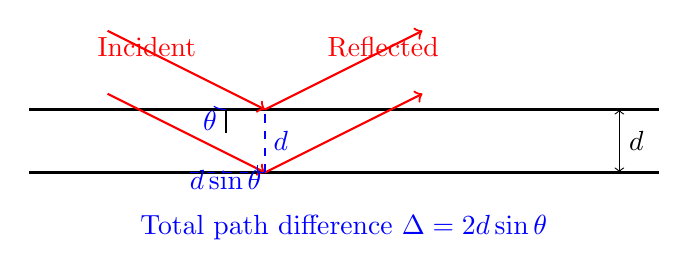
\begin{tikzpicture}[scale=1.0]
    % Draw crystal planes
    \draw[thick] (-4,0) -- (4,0);
    \draw[thick] (-4,-0.8) -- (4,-0.8);
    
    % Label d-spacing
    \draw[<->] (3.5,0) -- (3.5,-0.8) node[midway,right] {$d$};
    
    % Draw incident and reflected rays
    \draw[->,thick,red] (-3,1) -- (-1,0);
    \draw[->,thick,red] (-1,0) -- (1,1);
    \draw[->,thick,red] (-3,0.2) -- (-1,-0.8);
    \draw[->,thick,red] (-1,-0.8) -- (1,0.2);
    
    % Draw the path difference construction
    \draw[blue,dashed] (-1,-0.8) -- (-1,0);  % vertical line
    \draw[blue,dashed] (-1,-0.8) -- (-2,-0.8);  % horizontal line
    
    % Add right angle marker
    \draw[blue] (-1.1,-0.7) -- (-1.1,-0.8) -- (-1,-0.8);
    
    % Label the triangle sides
    \node[blue] at (-1.5,-0.9) {$d\sin\theta$};
    \node[blue] at (-0.8,-0.4) {$d$};
    
    % Draw angle θ from normal
    \draw[thick] (-1.5,0) -- (-1.5,-0.3);  % normal line
    \draw[blue] (-1.5,0) arc (270:240:0.3);
    \node[blue] at (-1.7,-0.15) {$\theta$};
    
    % Add labels
    \node[red] at (-2.5,0.8) {Incident};
    \node[red] at (0.5,0.8) {Reflected};
    
    % Add explanation
    \node[blue] at (0,-1.5) {Total path difference $\Delta = 2d\sin\theta$};
\end{tikzpicture}

Using Bragg's law: $2d\sin\theta = n\lambda$

\begin{parts}
\part
For the $a_1$ plane ($d = 0.468\text{ nm}$):
For n = 1: $\sin\theta = \frac{\lambda}{2a_1} = \frac{0.166}{2(0.468)} = 0.177$
Therefore $\theta = 10.2^\circ$ and $2\theta = 20.4^\circ$


\part
For the $a_2$ plane ($d = 0.342\text{ nm}$):
$\sin\theta = \frac{0.166}{2(0.342)} = 0.243$
Therefore $\theta = 14.1^\circ$ and $2\theta = 28.2^\circ$

Higher order reflections occur at:
n = 2: $2\theta = 2\arcsin(2 \times 0.243) = 58.9^\circ$
n = 3: $2\theta = 2\arcsin(3 \times 0.243) = 95.7^\circ$ (not visible in range)

\part
\begin{tikzpicture}[scale=0.1]
    % Draw axes
    \draw[->] (0,0) -- (90,0) node[right] {$2\theta$ ($^\circ$)};
    \draw[->] (0,0) -- (0,25) node[above] {Intensity};
    
    % Draw Bragg peaks for a1 (n=1,2,3)
    \draw[thick] (20.4,0) -- (20.4,20) node[above] {$a_1$};
    \draw[thick] (41.9,0) -- (41.9,10) node[above] {$2a_1$};
    \draw[thick] (65.1,0) -- (65.1,5) node[above] {$3a_1$};
    
    % Draw Bragg peaks for a2 (n=1,2)
    \draw[thick] (28.2,0) -- (28.2,20) node[above] {$a_2$};
    \draw[thick] (58.9,0) -- (58.9,10) node[above] {$2a_2$};
    
    % Add tick marks
    \foreach \x in {0,15,30,45,60,75,90}
        \draw (\x,0.2) -- (\x,-0.2) node[below] {\x};
\end{tikzpicture}

The intensity of higher-order reflections ($n > 1$) decreases due to several factors:
\begin{itemize}
    \item The atomic form factor $f(q)$ decreases with increasing scattering vector $q = 4\pi\sin\theta/\lambda$
    \item The Debye-Waller factor $e^{-M}$ reduces intensity more at higher angles due to thermal vibrations
    \item At larger angles, the geometric factor $\sin\theta$ in the denominator of the intensity formula becomes more significant
\end{itemize}
\end{parts}
\end{solution}
  
\miquestion
Metals and insulators. Explain the following:

\begin{parts}
    \part
sodium, which has two atoms in a bcc (conventional cubic) unit cell, is
    a metal.
\part
    calcium, which has four atoms in an fcc (conventional cubic) unit cell, is
    a metal.
\part
    diamond, which has eight atoms in an fcc (conventional cubic) unit cell, is
    an electrical insulator, whereas silicon and germanium, which have similar
    structures, are semiconductors.
    (Try to think up several possible reasons!)
\part
    Why is diamond transparent?
\part
    Why are metals not transparent?
\part
    Why are metals shiny?
\end{parts}

\begin{solution}
\begin{parts}
\part
Sodium (Na) is a metal because:
- Each Na atom contributes one 3s electron to the conduction band
- With 2 atoms per bcc unit cell, there are 2 electrons per unit cell
- The first Brillouin zone can hold 2 electrons (one of each spin)
- This partially filled band leads to metallic behavior

\part
Calcium (Ca) is a metal because:
- Each Ca atom contributes two 4s electrons to the conduction band
- With 4 atoms per fcc unit cell, there are 8 electrons per unit cell
- These electrons partially fill the bands, resulting in metallic behavior

\part
The differences between diamond, Si, and Ge can be explained by:
1. Bond strength: Diamond has stronger sp³ covalent bonds than Si or Ge
2. Band gap: Diamond (~5.5 eV) > Si (1.1 eV) > Ge (0.67 eV)
3. Lattice parameter differences affect orbital overlap
4. Core electron shielding increases down the group, affecting band structure

\part
Diamond is transparent because:
- Its large band gap (~5.5 eV) exceeds visible light energies (1.65-3.1 eV)
- Therefore visible photons cannot excite electrons across the gap

\part
Metals are not transparent because:
- Free electrons in the conduction band can absorb photons of any energy
- They also reflect most incident light due to plasma oscillations

\part
Metals are shiny because:
\begin{itemize}
\item Free electrons oscillate in response to incident electromagnetic waves
\item This creates a strong reflected wave (high reflectivity)
\item The reflection occurs across the entire visible spectrum
\item The plasma frequency $\omega_p = \sqrt{\frac{ne^2}{\epsilon_0 m}}$ is typically in the ultraviolet 
($\sim$10-15 eV for simple metals)
\item Light below the plasma frequency is reflected (visible light is $\sim$1.5-3 eV)
\item Above $\omega_p$, metals become transparent (this is why aluminum becomes transparent to X-rays)
\end{itemize}
\end{parts}
\end{solution}
  

\miquestion
Effective mass. 

Let us assume that in a semiconductor, we can describe the dispersion relation
as a Taylor expansion,

$E(k)=E_0 + \alpha |k-k_0|^2 + ...$

with $\alpha>0$ and $...$ being the higher order terms in the Taylor expansion
which we will ignore (harmonic approximation). 

We can then define the effective mass as

$\frac{\hbar^2}{2m^*} = \frac{\partial^2 E}{\partial k^2} = 2\alpha$.

Let us consider an electron near the top of the valence band in
a seminconductor with dispersion relation

    $E(k)=-10^{-37} |k|^2$,

where $E$ is in Joules, and $k$ is in $m^{-1}$. 

We remove an electron from state $k=2x10^{-8}$~m$^{-1} \hat x$, where $\hat x$ is
the unit vector in the $x$-direction. 

For a hole, calculate, and give the sign of:

\begin{parts}
    \part
the effective mass,
\part
the energy,
\part
the momentum,
\part
the crystal momentum (assume a lattice spacing of 1 nm),
\part
the velocity. 
\end{parts}

\begin{solution}
\begin{parts}
\part
Effective mass:
\begin{align*}
m^* &= -\frac{\hbar^2}{2\alpha} = -\frac{(1.055 \times 10^{-34})^2}{2(-10^{-37})} = 5.56 \times 10^{-31} \text{ kg} \\
&= \frac{5.56 \times 10^{-31}}{9.109 \times 10^{-31}} = 0.61 \, m_e
\end{align*}
(positive, as expected for a hole, and a reasonable value for a semiconductor)

\part
Energy:
\begin{align*}
E &= +10^{-37}|2\times10^8|^2 = 4 \times 10^{-21} \text{ J} \\
&= \frac{4 \times 10^{-21}}{1.602 \times 10^{-19}} = 0.025 \text{ eV}
\end{align*}
(positive, opposite to electron, and a typical thermal energy scale)

\part
Momentum:
\begin{align*}
p &= -\hbar k = -(1.055 \times 10^{-34})(2\times10^8) = -2.11 \times 10^{-26} \text{ kg}\cdot\text{m}/\text{s} \\
k &= 2\times10^8 \text{ m}^{-1}
\end{align*}
(opposite to electron)

\part
Crystal momentum:
\begin{itemize}
\item With 1 nm lattice spacing, the Brillouin zone boundary is at $k_\text{BZ} = \frac{\pi}{a} = \frac{\pi}{10^{-9}} = 3.14 \times 10^9 \text{ m}^{-1}$
\item Our $k = 2\times10^8 \text{ m}^{-1}$ is therefore $\approx 6.4\%$ of the way to the zone boundary
\item This justifies our use of the parabolic band approximation, as we are close to the zone center
\end{itemize}

\part
Velocity:
$v = \frac{1}{\hbar}\frac{\partial E}{\partial k} = \frac{2\times10^{-37}|k|}{\hbar} = 3.78 \times 10^3$ m/s
(same direction as electron)
\end{parts}
\end{solution}
  

\miquestion

Drude mobility theory. In the low density limit, such as the semiconductor
described above, the Drude transport equation (really just Newton's laws of
motion) is a good approximation, and can be written down as

$m^* a = m^* \frac{dv}{dt} = -e*E - m^* v / \tau$,

here $E$ is the electric field, $v$ the velocity, $e$ the charge of an
electron, and $\tau$ the scattering time. 

The mobility ($\mu$) is the ratio of the velocity to the electric field, and therefore 

$\mu = \frac{|v|}{|E|} = \frac{e\tau}{m^*}$

\begin{parts}
    \part Assuming a scattering time of 10~fs, calculate the mobility for the
    semiconductor above.

\end{parts}

\begin{solution}
\begin{parts}
\part
Using $\mu = \frac{e\tau}{m^*}$:

$\tau = 10\text{ fs} = 10^{-14}$ s
$e = 1.602 \times 10^{-19}$ C
$m^* = 5.56 \times 10^{-31}$ kg (from previous question)

Therefore:
\begin{align*}
\mu &= \frac{(1.602 \times 10^{-19})(10^{-14})}{5.56 \times 10^{-31}} \\
&= 0.00288 \text{ m}^2/(\text{V}\cdot\text{s}) \\
&= 28.8 \text{ cm}^2/(\text{V}\cdot\text{s})
\end{align*}

This is a reasonable mobility for a semiconductor at room temperature, comparable to silicon 
($\sim 1400 \text{ cm}^2/(\text{V}\cdot\text{s})$ for electrons, 
$\sim 450 \text{ cm}^2/(\text{V}\cdot\text{s})$ for holes).
\end{parts}
\end{solution}
  

%force a page break for better layout of questions 
%NOTE: only force pagebreaks at the final stage for perfecting the layout
%\newpage


\end{questions}

\end{document}
